\documentclass[12pt]{article}

\usepackage{graphicx}% Include figure files
\usepackage{dcolumn}% Align table columns on decimal point

% Use Arial font %
\usepackage{helvet}
\renewcommand{\familydefault}{\sfdefault} 

% Default margins and paper properties %
\usepackage[a4, portrait, margin=0.6in]{geometry}

\begin{document}
	\title{Hypothesis plots summary} % Force line breaks with \\
	\author{1666957, Gustavo Espinal Lugo}
	\date{\today} % It is always \today, today, %  but any date may be explicitly specified

	\maketitle
	%\tableofcontents
	
	\section*{Plots and corresponding metadata}
	Number of data points used: 99999,\\
mean expected W mass: 80.36010913 $[GeV/c^{2}]$,\\
mean hypothesis masses $[GeV/c^{2}]$: [<generator object <genexpr> at 0x7fd009d88510>],\\
mass width: 2.07041274 $[GeV/c^{2}]$,\\
chi\_square value of hypothesis fit: 146.67302655954285\\
	Absolute path to figure: /home/physics/phuxdp/Desktop/PX402 Physics Project/WBosonProject/noQED/plots/muPT\_80.36010913\_2.07041274\_between\_78\_and\_92.png\\
	Next lines are the data of the shown histograms (if needed): \\
	All quantities: 	99999, 80.36010913, [78.  79.4 80.8 82.2 83.6 85.  86.4 87.8 89.2 90.6 92. ], 2.07041274, 146.67302655954285\\
	X\_energ\_vls = [30.1, 30.299999999999997, 30.5, 30.700000000000003, 30.9, 31.1, 31.299999999999997, 31.5, 31.700000000000003, 31.9, 32.1, 32.3, 32.5, 32.7, 32.9, 33.1, 33.3, 33.5, 33.7, 33.9, 34.1, 34.3, 34.5, 34.7, 34.9, 35.1, 35.3, 35.5, 35.7, 35.9, 36.1, 36.3, 36.5, 36.7, 36.9, 37.1, 37.3, 37.5, 37.7, 37.9, 38.1, 38.3, 38.5, 38.7, 38.9, 39.1, 39.3, 39.5, 39.7, 39.9, 40.1, 40.3, 40.5, 40.7, 40.9, 41.1, 41.3, 41.5, 41.7, 41.9, 42.1, 42.3, 42.5, 42.7, 42.9, 43.1, 43.3, 43.5, 43.7, 43.9, 44.1, 44.3, 44.5, 44.7, 44.9, 45.1, 45.3, 45.5, 45.7, 45.9, 46.1, 46.300000000000004, 46.5, 46.7, 46.9, 47.1, 47.300000000000004, 47.5, 47.7, 47.9, 48.1, 48.300000000000004, 48.5, 48.7, 48.9, 49.1, 49.300000000000004, 49.5, 49.7, 49.9]\\
	Y\_data\_bin\_cnts = [266.0, 281.0, 301.0, 304.0, 281.0, 321.0, 336.0, 324.0, 300.0, 328.0, 328.0, 325.0, 318.0, 337.0, 328.0, 371.0, 345.0, 331.0, 383.0, 356.0, 327.0, 345.0, 368.0, 354.0, 369.0, 369.0, 367.0, 344.0, 389.0, 342.0, 384.0, 374.0, 371.0, 385.0, 365.0, 370.0, 364.0, 348.0, 351.0, 340.0, 420.0, 408.0, 389.0, 399.0, 403.0, 398.0, 377.0, 376.0, 348.0, 319.0, 320.0, 307.0, 319.0, 305.0, 286.0, 320.0, 272.0, 260.0, 239.0, 235.0, 228.0, 215.0, 216.0, 211.0, 204.0, 180.0, 196.0, 185.0, 158.0, 154.0, 148.0, 127.0, 134.0, 128.0, 120.0, 120.0, 123.0, 101.0, 104.0, 94.0, 110.0, 105.0, 81.0, 79.0, 100.0, 86.0, 75.0, 76.0, 86.0, 83.0, 80.0, 77.0, 65.0, 70.0, 73.0, 61.0, 64.0, 56.0, 57.0, 66.0]\\
	Y\_model\_bin\_cnts = [313.2992858886719, 106.21347045898438, 345.7534484863281, 282.5838317871094, 83.59107971191406, 193.91091918945312, 288.21978759765625, 23.846467971801758, 176.83392333984375, 279.2972106933594, 58.44918441772461, 83.54625701904297, 255.6328582763672, 381.4120788574219, 181.0519256591797, 89.92611694335938, 36.13596725463867, 116.2718505859375, 47.71955490112305, 330.4010925292969, 58.3175048828125, 407.54644775390625, 219.49285888671875, 296.8296203613281, 95.50274658203125, 239.26370239257812, 362.90301513671875, 425.0135498046875, 68.96009826660156, 65.85767364501953, 69.5289077758789, 203.36705017089844, 109.0361557006836, 486.18792724609375, 161.3716583251953, 136.0915985107422, 190.7365264892578, 414.1539001464844, 120.77681732177734, 153.4157257080078, 116.39080047607422, 150.96006774902344, 356.43096923828125, 215.05323791503906, 310.41192626953125, 577.3638916015625, 315.0453186035156, 597.8947143554688, 420.2438049316406, 112.79922485351562, 265.34747314453125, 120.4859390258789, 354.1427307128906, 171.23988342285156, 429.74530029296875, 740.4324340820312, 269.5274658203125, 98.54425811767578, 343.9665222167969, 439.8898620605469, 160.5813751220703, 222.04930114746094, 369.69537353515625, 200.85897827148438, 269.5789794921875, 328.0943908691406, 210.26858520507812, 223.17535400390625, 321.5649719238281, 293.3818664550781, 352.95892333984375, 465.11041259765625, 347.0108947753906, 409.08746337890625, 187.93934631347656, 59.240638732910156, 409.1673889160156, 113.01419067382812, 175.86167907714844, 71.2312240600586, 315.273681640625, 128.443115234375, 168.57762145996094, 235.40316772460938, 132.71621704101562, 232.0699920654297, 344.87786865234375, 20.746023178100586, 384.71148681640625, 218.5894317626953, 187.9745330810547, 158.18234252929688, 25.815486907958984, 256.2192077636719, 223.65428161621094, 122.94083404541016, 154.239501953125, 62.06776428222656, 32.254478454589844, 43.664268493652344]\\

    Found optimal massses ($\chi^2$ roots): [80.4783045] $[GeV/c^{2}]$\\
    Uncertainty [GeV/c^2]: 0.0\\

	\begin{figure}[tb]
		\centering
		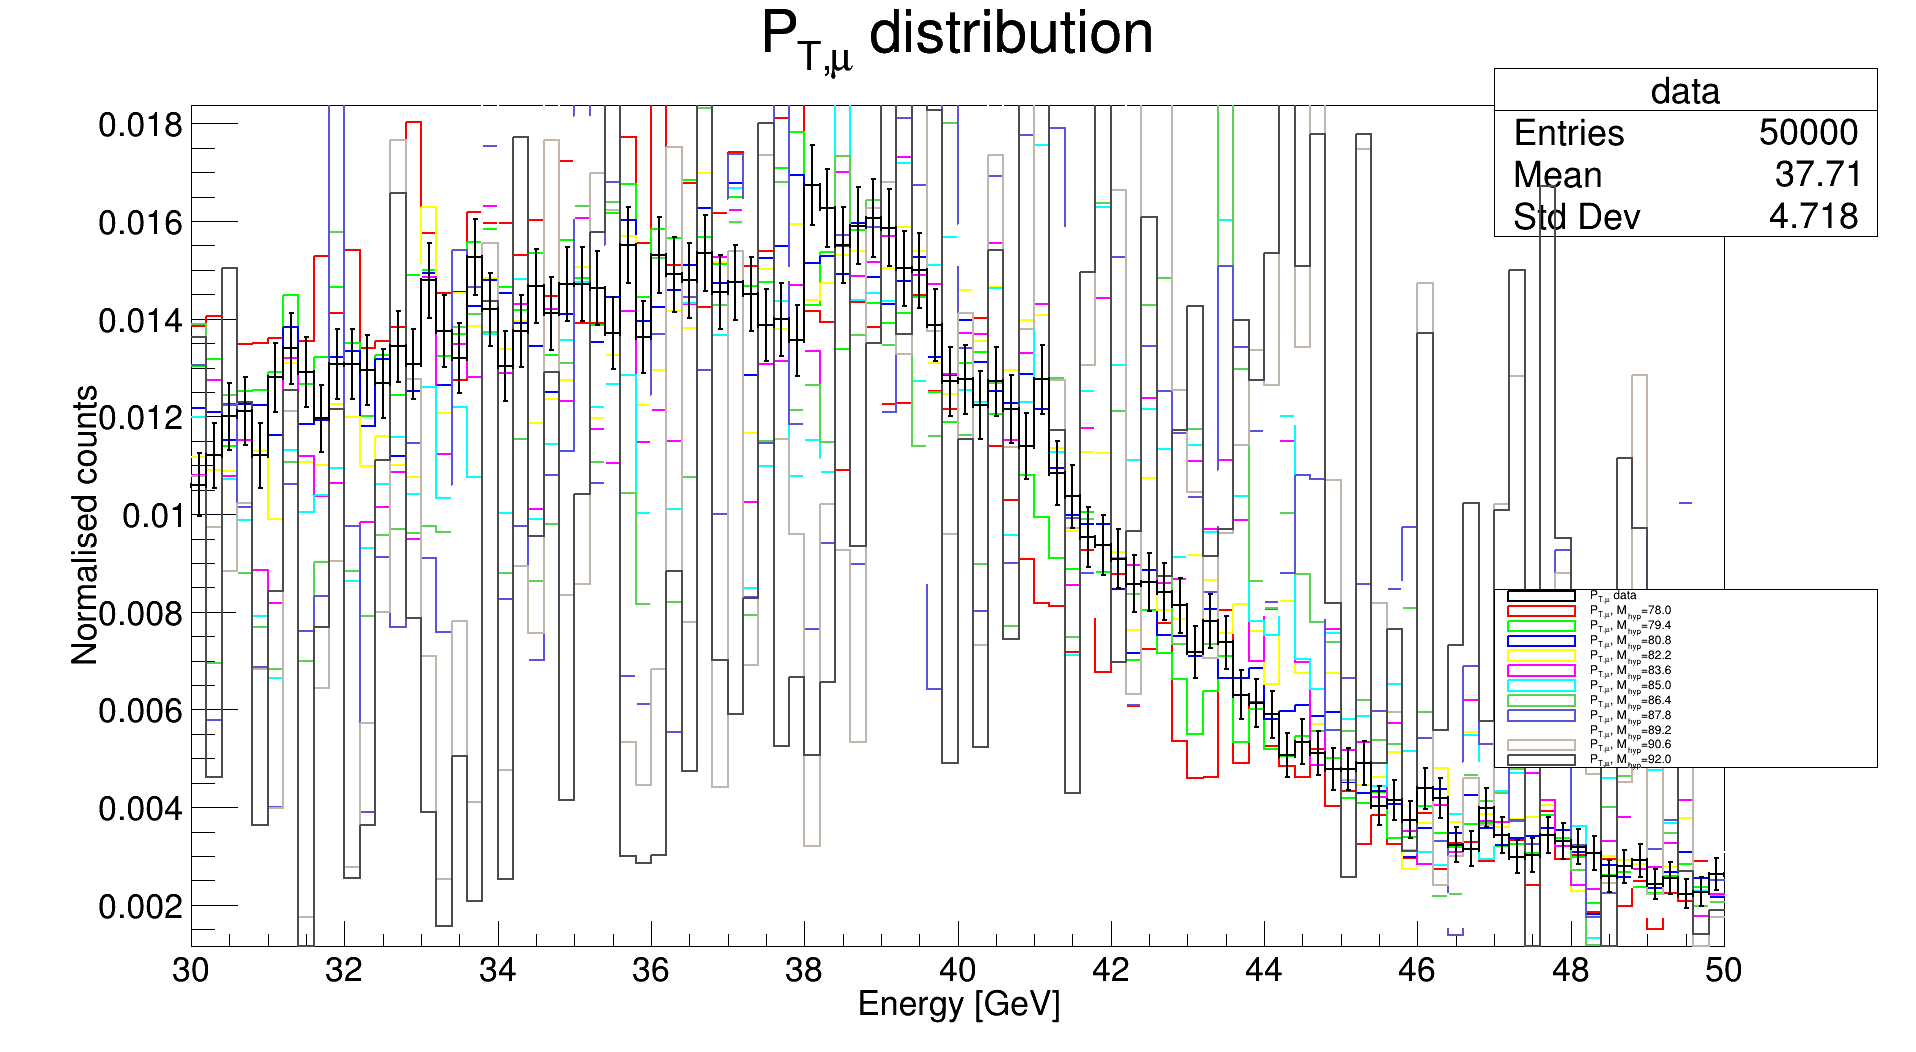
\includegraphics[width=\columnwidth]{/home/physics/phuxdp/Desktop/PX402 Physics Project/WBosonProject/noQED/plots/muPT_80.36010913_2.07041274_between_78_and_92.png}
		\caption{\small Hypothesis masses Number of data points used: 99999,\\
mean expected W mass: 80.36010913 $[GeV/c^{2}]$,\\
mean hypothesis masses $[GeV/c^{2}]$: [<generator object <genexpr> at 0x7fd009d88510>],\\
mass width: 2.07041274 $[GeV/c^{2}]$,\\
chi_square value of hypothesis fit: 146.67302655954285. }
		\label{fig: fig_0}
	\end{figure}
    Notes: \\
    1) Using mu\_born\_PT as pseudodata and  Mu\_Pt as model/hypothesis\\
    2) Using full run mode\\
       \begin{figure}[tb]
		\centering
		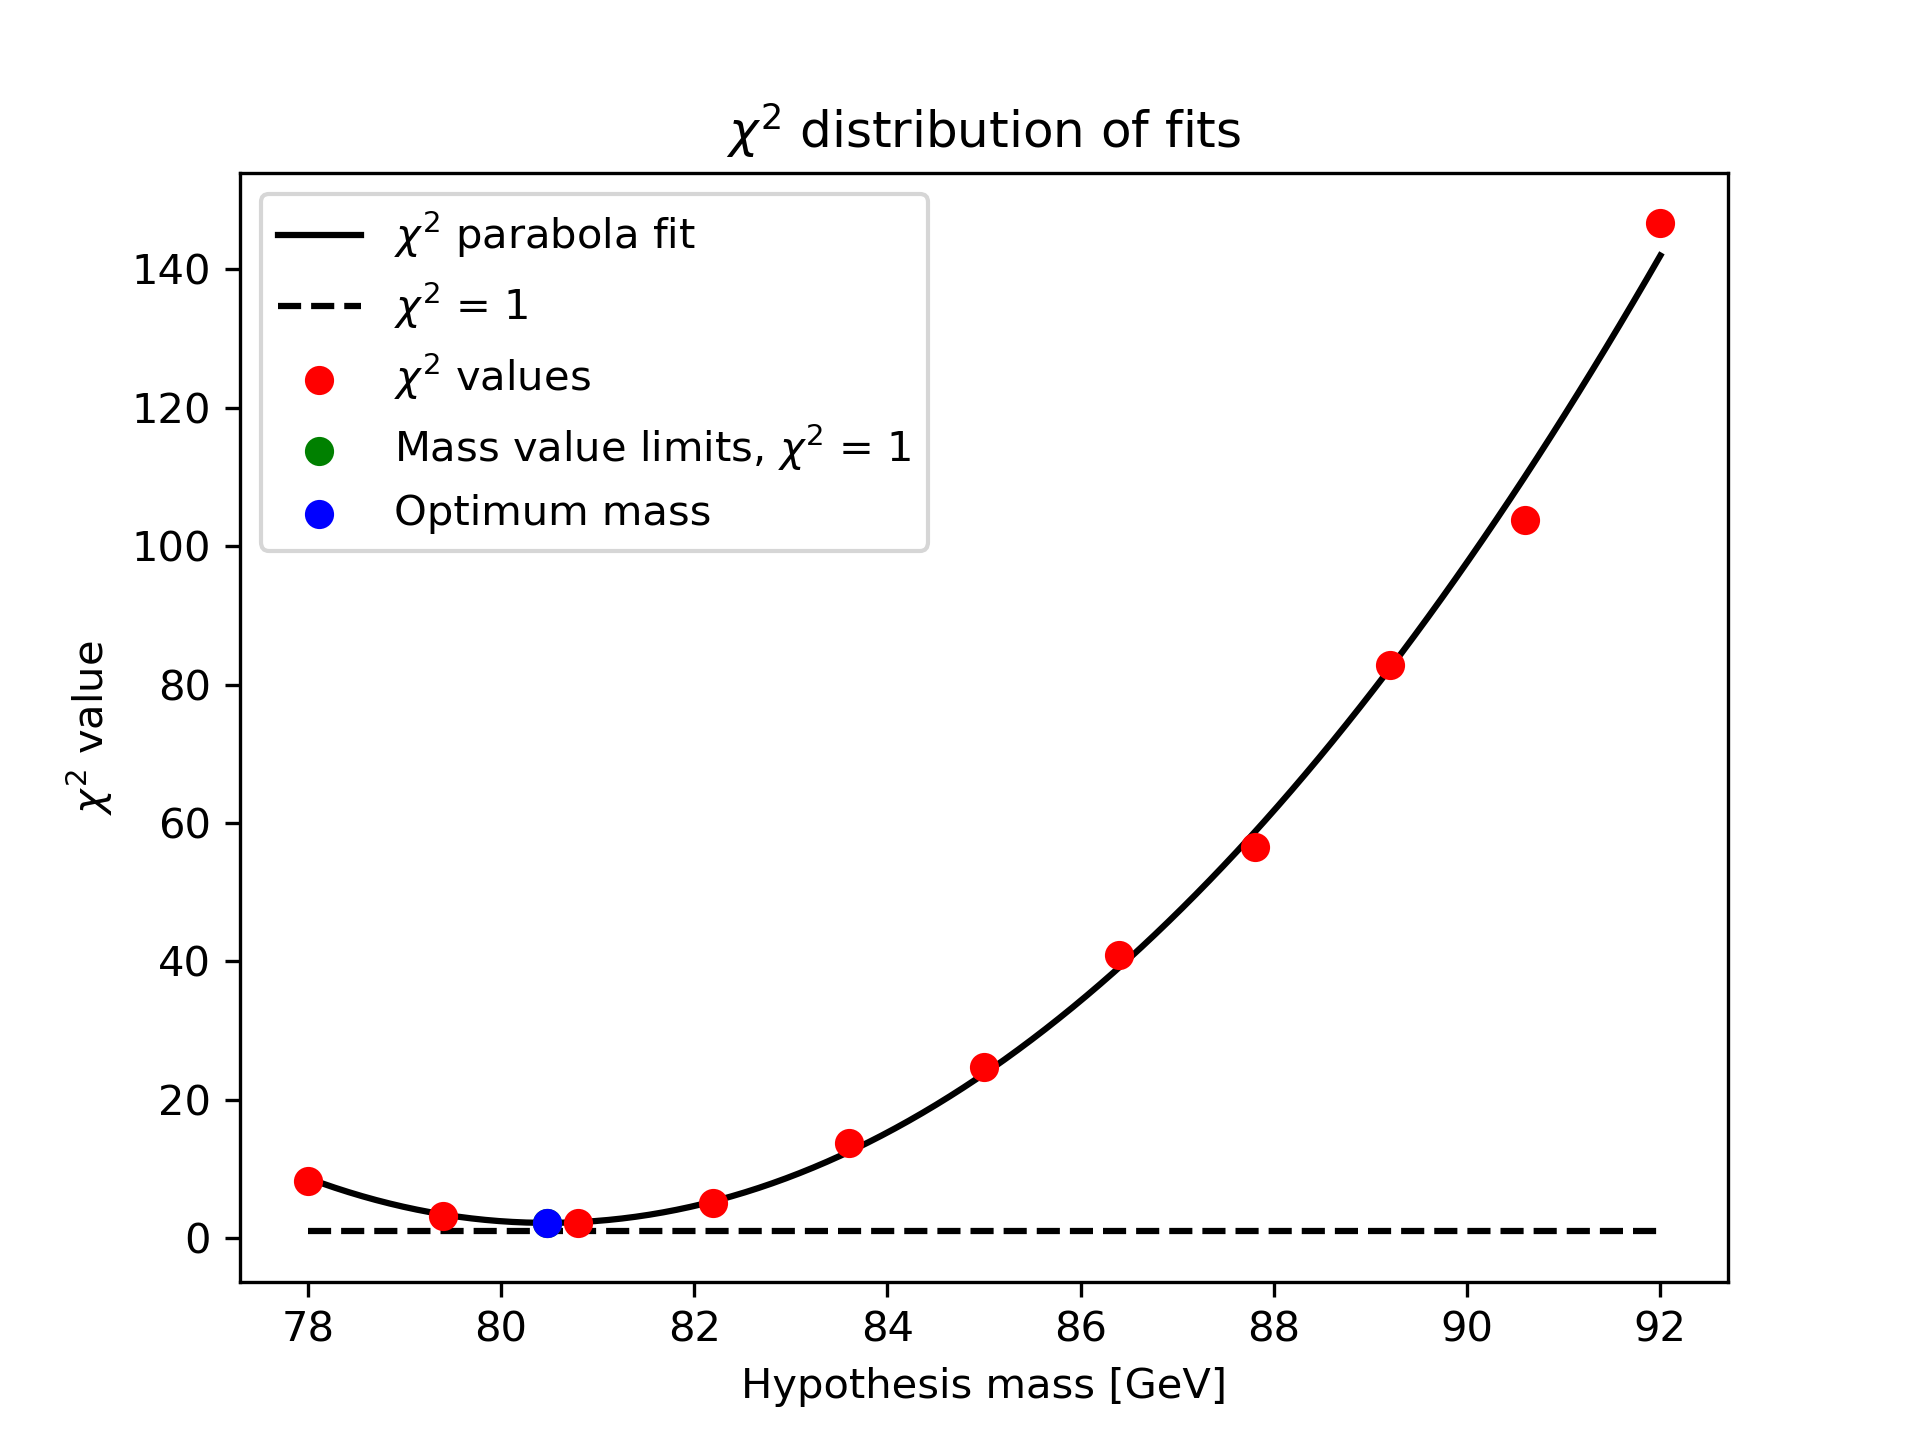
\includegraphics[width=\columnwidth]{/home/physics/phuxdp/Desktop/PX402 Physics Project/WBosonProject/noQED/plots/chi_square_fits_muPT_80.36010913_2.07041274_between_78_and_92.png}
		\caption{\small $\chi^2$ of hypothesis masses. }
		\label{fig: fig_chi_square}
	\end{figure}

    \begin{figure}[tb]
		\centering
		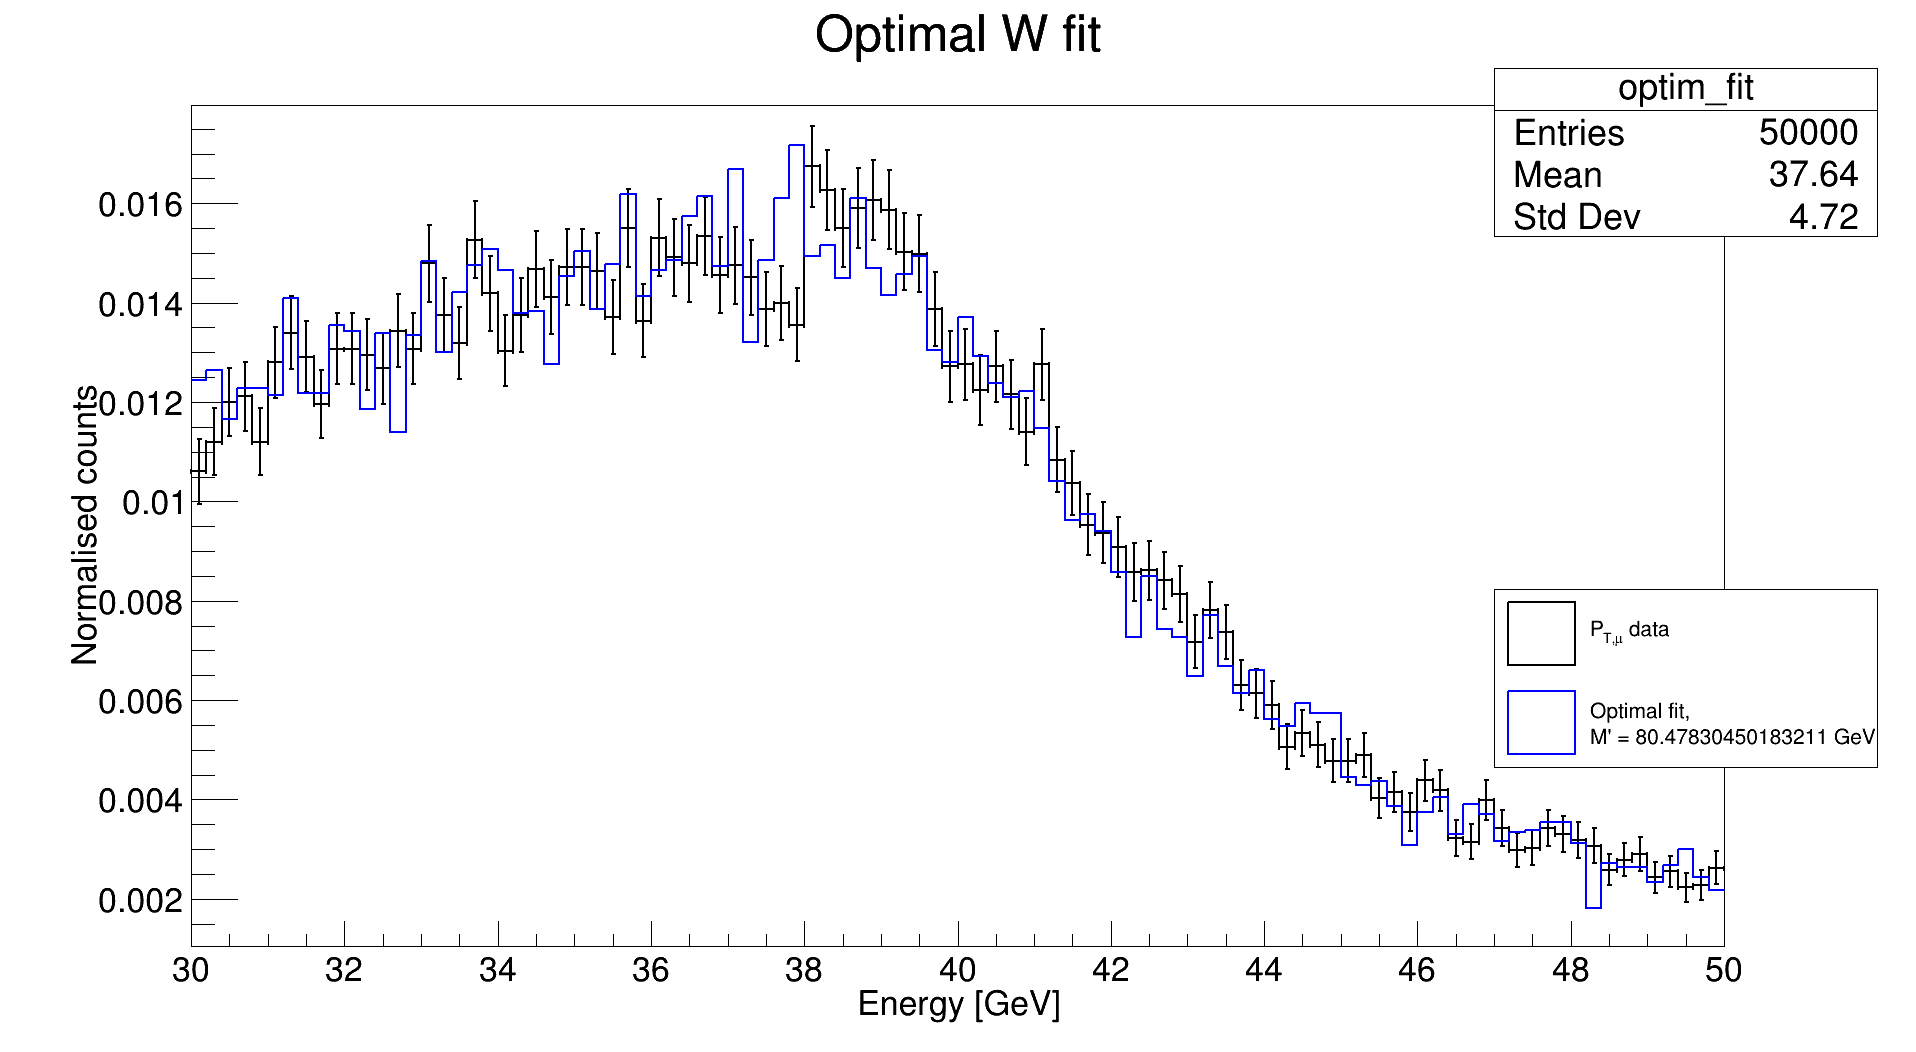
\includegraphics[width=\columnwidth]{/home/physics/phuxdp/Desktop/PX402 Physics Project/WBosonProject/noQED/plots/optimum_muPT_80.36010913_2.07041274_between_78_and_92.png}
		\caption{\small Data and optimum fit with $\chi^2 = 2.1776366388229618$. Used the hypothesis mass of 80.47830450183211 $[GeV/c^{2}]$. }
		\label{fig: fig_optim_parms}
	\end{figure}
    
\end{document}